\chapter{Linear Models}

Reality is too complex. Our mind, no matter how powerful it is, can't keep track of all the messy details that result in some outcome. For example, if you want to understand how fast the car will move when you hit the pedal - you don't want to track every molecule of gasoline, energy released when it's combusted, displacement of the engine's piston, and so on. Instead, we need a simplified version of this reality. We just want to know the relation between \textit{how fast the car goes} and \textit{how hard the pedal is pressed}. This is known as \textit{modelling}.\\

\textit{Why do we care about modelling?} Because it helps us: 

\begin{itemize}
    \item \textbf{Understand}: When you can model something, you grasp the big picture. You know what variables matter and how they interact.
    \item \textbf{Predict}: If you can model the weather, the stock market, or disease spread, you can forecast the future, or at least get close!
    \item \textbf{Control}: Once you understand how things work through a model, you can make decisions to steer the outcome the way you want.
\end{itemize}

\section{Introduction to Statistical Modelling}

Suppose we want to understand \textit{how much rainfall do we expect to get} on a particular day. We denote this \textbf{quantitative} variable as $Y$. Next, we make an assumption of what all parameters impact our variable $Y$. In this case, it could be \textit{temperature, humidity, wind speed, month of the year,} and so on. If our assumption is wrong, we will come to know about that during our analysis and modelling process. So, we can safely assume that there are $p$ measureable predictors that impact $Y$ and could be denoted by $X_1$, $X_2$, $X_3$,...,$X_p$.  Let $X$ be the set of all these predictors: $X = (X_1, X_2, X_3, ..., X_p)$. We want to find the \textbf{unknown} function $f$ such that

\[
Y = f(X) + \epsilon
\]

where $\epsilon$ is the error term. \textit{Why do we have an error term?} Because even the best models can’t capture every tiny detail of reality. There’s always some randomness, some noise, or some missing information. Epsilon accounts for all the stuff we don't know, couldn’t measure or predict.\\

Usually, we have some historic measurements of $Y$ and the corresponding values of $X$. By looking at these measurements, we try to come up with a function $\hat{f}$ which is an estimate of the original unknown function $f$. This will give us $\hat{Y}$, our prediction/estimate of the $Y$. 

\[
\hat{Y} = \hat{f}(X)
\]

We still don't know how we will come up with this $\hat{f}$ function. For us, it is a \textit{black box}, in the sense that one is not typically concerned with the exact form of $\hat{f}$, provided that it yields accurate predictions for $Y$.\cite{islr}\\

The accuracy of $\hat{Y}$ as an estimate for $Y$ relies on two main sources of error: the \textit{reducible error} and the \textit{irreducible error}. Generally, $\hat{f}$, which is our estimate of $f$, is not perfect, leading to some inaccuracies. This discrepancy contributes to the \textit{reducible error} because it can potentially be minimized by selecting a more suitable statistical learning method to estimate $f$. \\

However, even if we could perfectly estimate $f$ so that our prediction is $\hat{Y} = f(X)$, there would still be some inherent error present. This is because $Y$ depends not only on $f(X)$ but also on a random error term, $\epsilon$, which by its nature cannot be predicted using $X$. The uncertainty introduced by $\epsilon$ affects the accuracy of our predictions, and this is referred to as the \textit{irreducible error}, as it cannot be reduced, regardless of how accurately we estimate $f$.\\

Why is the irreducible error greater than zero? The term $\epsilon$ may contain unobserved variables that could help in predicting $Y$; since these variables are not measured, $f$ cannot utilize them for prediction. Additionally, $\epsilon$ may also account for random variation that cannot be measured. For instance, a patient’s risk of an adverse reaction could vary from day to day based on variations in the drug’s manufacturing process or the patient’s overall health status.\\

Now, consider an estimate $\hat{f}$ and a set of predictors $X$ which yield the prediction $\hat{Y} = \hat{f}(X)$. Assume that $\hat{f}$ and $X$ are fixed for a moment. Then, we can express the expected squared error as follows:

\begin{equation}
    E[(Y - \hat{Y})^2] = E[(f(X) + \epsilon - \hat{f}(X))^2] = [f(X) - \hat{f}(X)]^2 + \text{Var}(\epsilon)
\end{equation}
\vspace{3pt}

Here, $E[(Y - \hat{Y})^2]$ denotes the expected value of the squared difference between the predicted and actual values of $Y$, which is also called the mean squared error (MSE). The term $\text{Var}(\epsilon)$ represents the variance of the error term $\epsilon$. \\

The focus of this discussion is on methods to estimate $f$ with the goal of minimizing the reducible error. However, it is crucial to remember that the irreducible error sets an upper limit on the accuracy of our predictions for $Y$. This upper bound is often unknown in practice.\\

\subsection{How to estimate $\hat{f}$}\cite{islr}

Throughout this book, we discuss various linear and non-linear techniques for estimating the function $f$. Although these methods differ, they tend to share some common features, which we will outline in this section. We assume that we have observed a collection of $n$ data points. These observations are known as the \textit{training data} because they are used to train or teach our method to estimate the function $f$. Let $x_{ij}$ denote the value of the $j$th predictor (or input) for the $i$th observation, where $i = 1, 2, \ldots, n$ and $j = 1, 2, \ldots, p$. Let $y_i$ represent the response variable for the $i$th observation. Thus, our training data can be expressed as:

\[
\{(x_1, y_1), (x_2, y_2), \ldots, (x_n, y_n)\}
\]

where $x_i = (x_{i1}, x_{i2}, \ldots, x_{ip})^T$. Our objective is to apply a statistical learning method to this training data to estimate the unknown function $f$. In essence, we aim to find a function $\hat{f}$ such that $Y \approx \hat{f}(X)$ for any new observation $(X, Y)$. Generally, most statistical learning approaches for this task fall into one of two categories: \textit{parametric} or \textit{non-parametric}.

\subsubsection{Parametric Methods}

Parametric methods rely on a two-step model-based process:

\begin{enumerate}
    \item \textbf{Assume a Functional Form}: We start by making an assumption about the form or structure of $f$. For instance, a straightforward assumption is that $f$ is linear in $X$, leading to a model of the form:

    \[
    f(X) = \beta_0 + \beta_1 X_1 + \beta_2 X_2 + \ldots + \beta_p X_p
    \]

    This is known as a linear model, which we will explore in detail throughout this book. By assuming $f$ is linear, the task of estimating $f$ becomes much simpler. Instead of estimating an entirely arbitrary function in a $p$-dimensional space, we now only need to estimate $p + 1$ coefficients: $\beta_0, \beta_1, \ldots, \beta_p$.

    \item \textbf{Fitting the Model}: Once the model form is selected, the next step involves fitting or training the model using the training data. In the case of the linear model mentioned above, we need to estimate the parameters $\beta_0, \beta_1, \ldots, \beta_p$ in such a way that:

    \[
    Y \approx \beta_0 + \beta_1 X_1 + \beta_2 X_2 + \ldots + \beta_p X_p
    \]

    The most common method for fitting such a model is \textit{ordinary least squares}. This approach minimizes the squared differences between the observed values and the values predicted by the model. However, ordinary least squares is just one way to fit a linear model; there are several alternative methods depending on the problem.
\end{enumerate}

The parametric approach described reduces the problem of estimating $f$ to estimating a finite set of parameters. By assuming a specific form for $f$, the estimation process becomes more manageable, as it typically involves fewer variables. However, a significant drawback of this approach is that the model chosen might not align closely with the true underlying function $f$. If the assumed model is too restrictive or too far from reality, our estimate will not be accurate. To mitigate this, we can opt for more flexible parametric models that capture a wider range of possible functional forms for $f$. Nevertheless, increasing the flexibility of a model generally requires estimating more parameters, which can lead to \textit{overfitting}. Overfitting occurs when the model captures the noise in the training data rather than the actual underlying pattern, leading to poor performance on new, unseen data.

\subsubsection{Non-parametric Methods}

Non-parametric methods take a different approach by avoiding explicit assumptions about the functional form of $f$. Instead, these methods aim to estimate $f$ directly from the data, adjusting to fit the data points as closely as possible without becoming overly complex or erratic. One of the major advantages of non-parametric methods is that they offer the flexibility to fit a broad range of shapes for $f$. By not imposing a specific form, these methods can potentially provide a more accurate estimate, particularly when the true function $f$ is complex or unknown.\\

However, this flexibility comes at a cost. Because non-parametric methods do not simplify the problem to a set of parameters, they typically require a much larger number of observations compared to parametric methods in order to produce a reliable estimate. Essentially, they need a rich dataset to accurately capture the patterns in the data without resorting to assumptions about the functional form of $f$.

\subsection{Measuring the Quality of the Model}

In modelling, the Mean Squared Error (MSE) is a fundamental measure used to assess the performance of models. It quantifies the average squared difference between the actual values and the predicted values. Specifically, the MSE is defined as:

\[
\text{MSE} = \frac{1}{n} \sum_{i=1}^{n} (y_i - \hat{y}_i)^2
\]

where \( y_i \) are the observed values, \( \hat{y}_i \) are the predicted values, and \( n \) is the number of observations. To evaluate the effectiveness of a model, it is common practice to split the data into two parts: the training set and the test set. The MSE calculated using these two subsets is referred to as the \textit{Training MSE} and \textit{Test MSE}, respectively.\\

\textbf{Training MSE} measures how well a model fits the data it was trained on. It is the average squared error computed using the training dataset. On the other hand, \textbf{Test MSE} evaluates the model's performance on unseen data, providing insight into how the model is expected to perform in practice.\\

As a general rule, \textit{the training MSE will decrease as the complexity (or flexibility) of the model increases}. When the model becomes more flexible, it can fit the training data more closely. In other words, a highly flexible model is capable of capturing the intricate details and patterns of the training dataset, resulting in a lower training MSE.\\

However, the test MSE may not necessarily decrease as model flexibility increases. In fact, it might initially decrease but will eventually increase, forming what is known as a \textbf{U-shape} curve. This phenomenon occurs due to the concept of \textbf{overfitting}.

\subsubsection{The U-Shape Curve of Test MSE}

When a model is overly complex, it can fit the noise and peculiarities in the training data rather than the true underlying patterns. This situation leads to a scenario where the \textit{Training MSE} is very low, but the \textit{Test MSE} is high. This discrepancy indicates that the model has memorized the training data rather than learning a generalizable pattern. We say the model is \textbf{overfit}.\\

The U-shape of the test MSE can be explained as follows: 

\begin{itemize}
    \item When the model is \textit{underfitting} (i.e., it is too simple to capture the relationship between the predictors and the response), both the training and test MSEs are high.
    \item As we increase the flexibility of the model, it starts capturing more of the pattern, causing the training MSE and test MSE to drop.
    \item However, if we continue to increase the flexibility, the model becomes so attuned to the training data that it loses its ability to generalize. Consequently, the \textit{test MSE} rises, while the \textit{training MSE} continues to fall.
\end{itemize}

The following plot shows the relationship between the training and test MSE as model flexibility increases. The training MSE steadily decreases as the model becomes more flexible, while the test MSE initially decreases but eventually rises, forming a U-shape.

\begin{center}
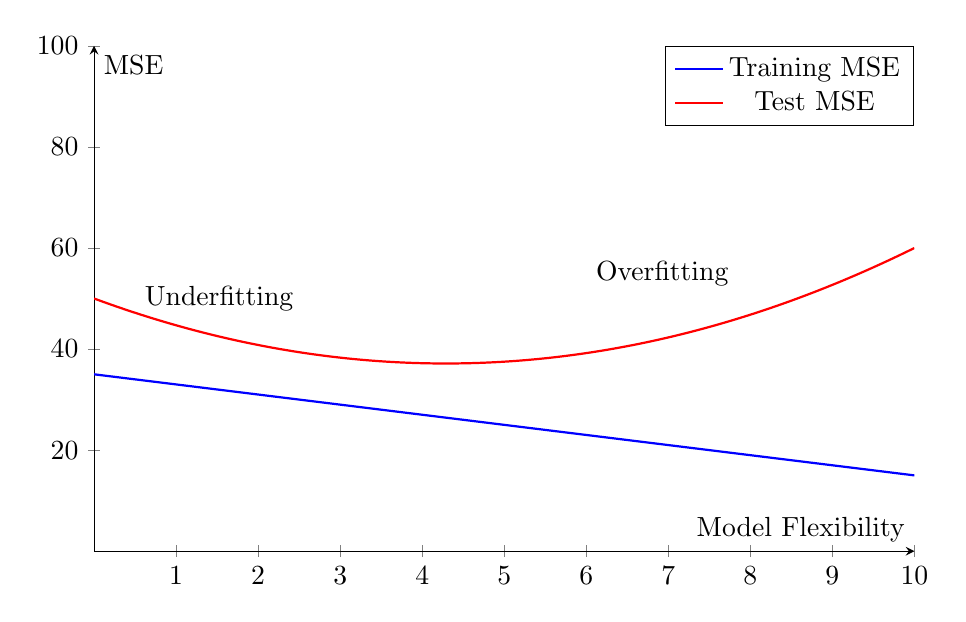
\begin{tikzpicture}
    \begin{axis}[
        xlabel={Model Flexibility},
        ylabel={MSE},
        ymin=0,
        xmin=0,
        xmax=10,
        ymax=100,
        legend style={at={(1,1)}, anchor=north east},
        domain=0:10,
        samples=100,
        axis x line=middle,
        axis y line=middle,
        width=12cm,
        height=8cm,
    ]
    % Training MSE curve
    \addplot [
        domain=0:10,
        smooth,
        thick,
        blue
    ] {35 - 2*x};
    \addlegendentry{Training MSE}

    % Test MSE curve
    \addplot [
        domain=0:10,
        smooth,
        thick,
        red
    ] {50 - 6*x + 0.7*x^2};
    \addlegendentry{Test MSE}

    % Annotations
    \node at (axis cs: 0.5,50) [anchor=west] {Underfitting};
    \node at (axis cs: 6,55) [anchor=west] {Overfitting};

    \end{axis}
\end{tikzpicture}
\end{center}

An important concept related to the train and test MSE is \textbf{variability}, or the sensitivity of a model to changes in the training data. A flexible model has higher variability, meaning it can change drastically with slight variations in the dataset. This makes it more likely to fit the noise in the data rather than the underlying pattern.\\

For example, if you were trying to predict house prices based on features like the number of bedrooms, location, and age of the house, a simple model might just give you a rough average price based on the number of bedrooms. While it may not be perfect, it would be relatively stable. In contrast, a very flexible model might try to fit every single fluctuation in price, even if those fluctuations are random or due to factors you haven’t measured. This model would perform extremely well on the training data but poorly on the test data because it would struggle with new, unseen examples that don't fit the training patterns precisely.

\subsection{Bias-Variance Trade Off}

Understanding the sources of error is critical for building models that generalize well to new data. One of the key concepts in this regard is the \textbf{bias-variance tradeoff}. It explains the balance between two sources of error that affect the performance of a model: \textbf{bias} and \textbf{variance}. These components together, along with irreducible error, make up the total prediction error. We express this relationship with the following equation:

\[
\mathbb{E} \left[ (y_0 - \hat{f}(x_0))^2 \right] = \text{Var}(\hat{f}(x_0)) + [\text{Bias}(\hat{f}(x_0))]^2 + \text{Var}(\epsilon)
\]

where:\\
 \( y_0 \) is the true output value at a new point \( x_0 \),\\
 \( \hat{f}(x_0) \) is the predicted value from the model at \( x_0 \),\\
 \( \text{Var}(\hat{f}(x_0)) \) is the variance of the model predictions at \( x_0 \),\\
 \( \text{Bias}(\hat{f}(x_0)) \) represents the bias of the model at \( x_0 \),\\
 \( \text{Var}(\epsilon) \) is the irreducible error, representing noise in the system that cannot be eliminated.

\subsubsection{Bias}

\textit{Bias} refers to the error introduced when the model oversimplifies the relationship between the predictors \( X \) and the response \( Y \). A model with high bias pays little attention to the details and patterns in the data, leading to inaccurate predictions. This typically happens when the model is too rigid or has low flexibility. In other words, it makes strong assumptions about the form of the relationship, like assuming a linear pattern when the actual relationship might be more complex.\\

An example of high bias is using a linear model to predict a highly non-linear relationship, such as trying to fit a straight line through data that clearly forms a parabolic pattern. Such a model will consistently miss the target values, resulting in a systematic error.\\

The squared bias term in the equation, \( [\text{Bias}(\hat{f}(x_0))]^2 \), measures the extent to which the average prediction of the model differs from the true value. High bias means the model is \textit{underfitting} the data.

\subsubsection{Variance}

\textit{Variance} refers to the model's sensitivity to small fluctuations in the training data. A model with high variance is overly complex and captures not just the underlying pattern but also the random noise in the training set. This leads to inconsistency when the model is applied to new, unseen data, as it produces vastly different outputs depending on the training data used.\\

Imagine a situation where you use a very flexible model, like a polynomial of high degree, to fit a dataset. The model will fit the training data almost perfectly, but if you change the training data slightly, the model's predictions could change drastically. This high sensitivity indicates that the model is not learning the general pattern but is instead learning the noise specific to the training data.\\

The term \( \text{Var}(\hat{f}(x_0)) \) in the equation represents this variability in the model's prediction at \( x_0 \). High variance means the model is \textit{overfitting} the data.

\subsubsection{The Bias-Variance Trade Off}

As we increase model flexibility, bias typically decreases because the model becomes capable of fitting more complex patterns. However, variance increases as the model starts capturing more noise from the training data. The goal is to find the \textbf{sweet spot} where the model is sufficiently complex to capture the underlying structure but not so flexible that it fits the noise. This is the point where the sum of bias and variance is minimized.\\

The term \( \text{Var}(\epsilon) \) in the equation represents the irreducible error or noise inherent in the system. No matter how well a model is designed, this error cannot be eliminated because it arises from factors beyond our control or measurement error in the observations.

\section{Simple Linear Regression}

In this discussion, we will explore simple linear regression using \href{https://raw.githubusercontent.com/MSc-Books/Generalised-Regression-Models/refs/heads/main/chapters/chapter1/data/placement.csv}{a dataset} containing two columns: CGPA (Cumulative Grade Point Average), denoted as \(X_1\), and the salary package, denoted as \(Y\). The CGPA is measured on a scale of 10, while the salary package is expressed in millions of Indian Rupees (INR) per annum. To visualize the relationship between CGPA and salary package, we can create a scatter plot [\ref{fig:scatter_plot_cgpa_salary}]. This plot reveals a positive linear correlation, suggesting that higher CGPA values are associated with higher salary packages. Based on this observation, we can formulate a linear model represented by the equation:

\[
Y \approx \beta_0 + \beta_1 X_1
\]

In this equation, \(Y\) is the dependent variable (salary package), and \(X_1\) is the independent variable (CGPA). The parameters \(\beta_0\) and \(\beta_1\) are unknown constants that correspond to the intercept and slope of the linear model, respectively. Together, these parameters are known as the model coefficients.\\

\begin{figure}[h!]
    \centering
    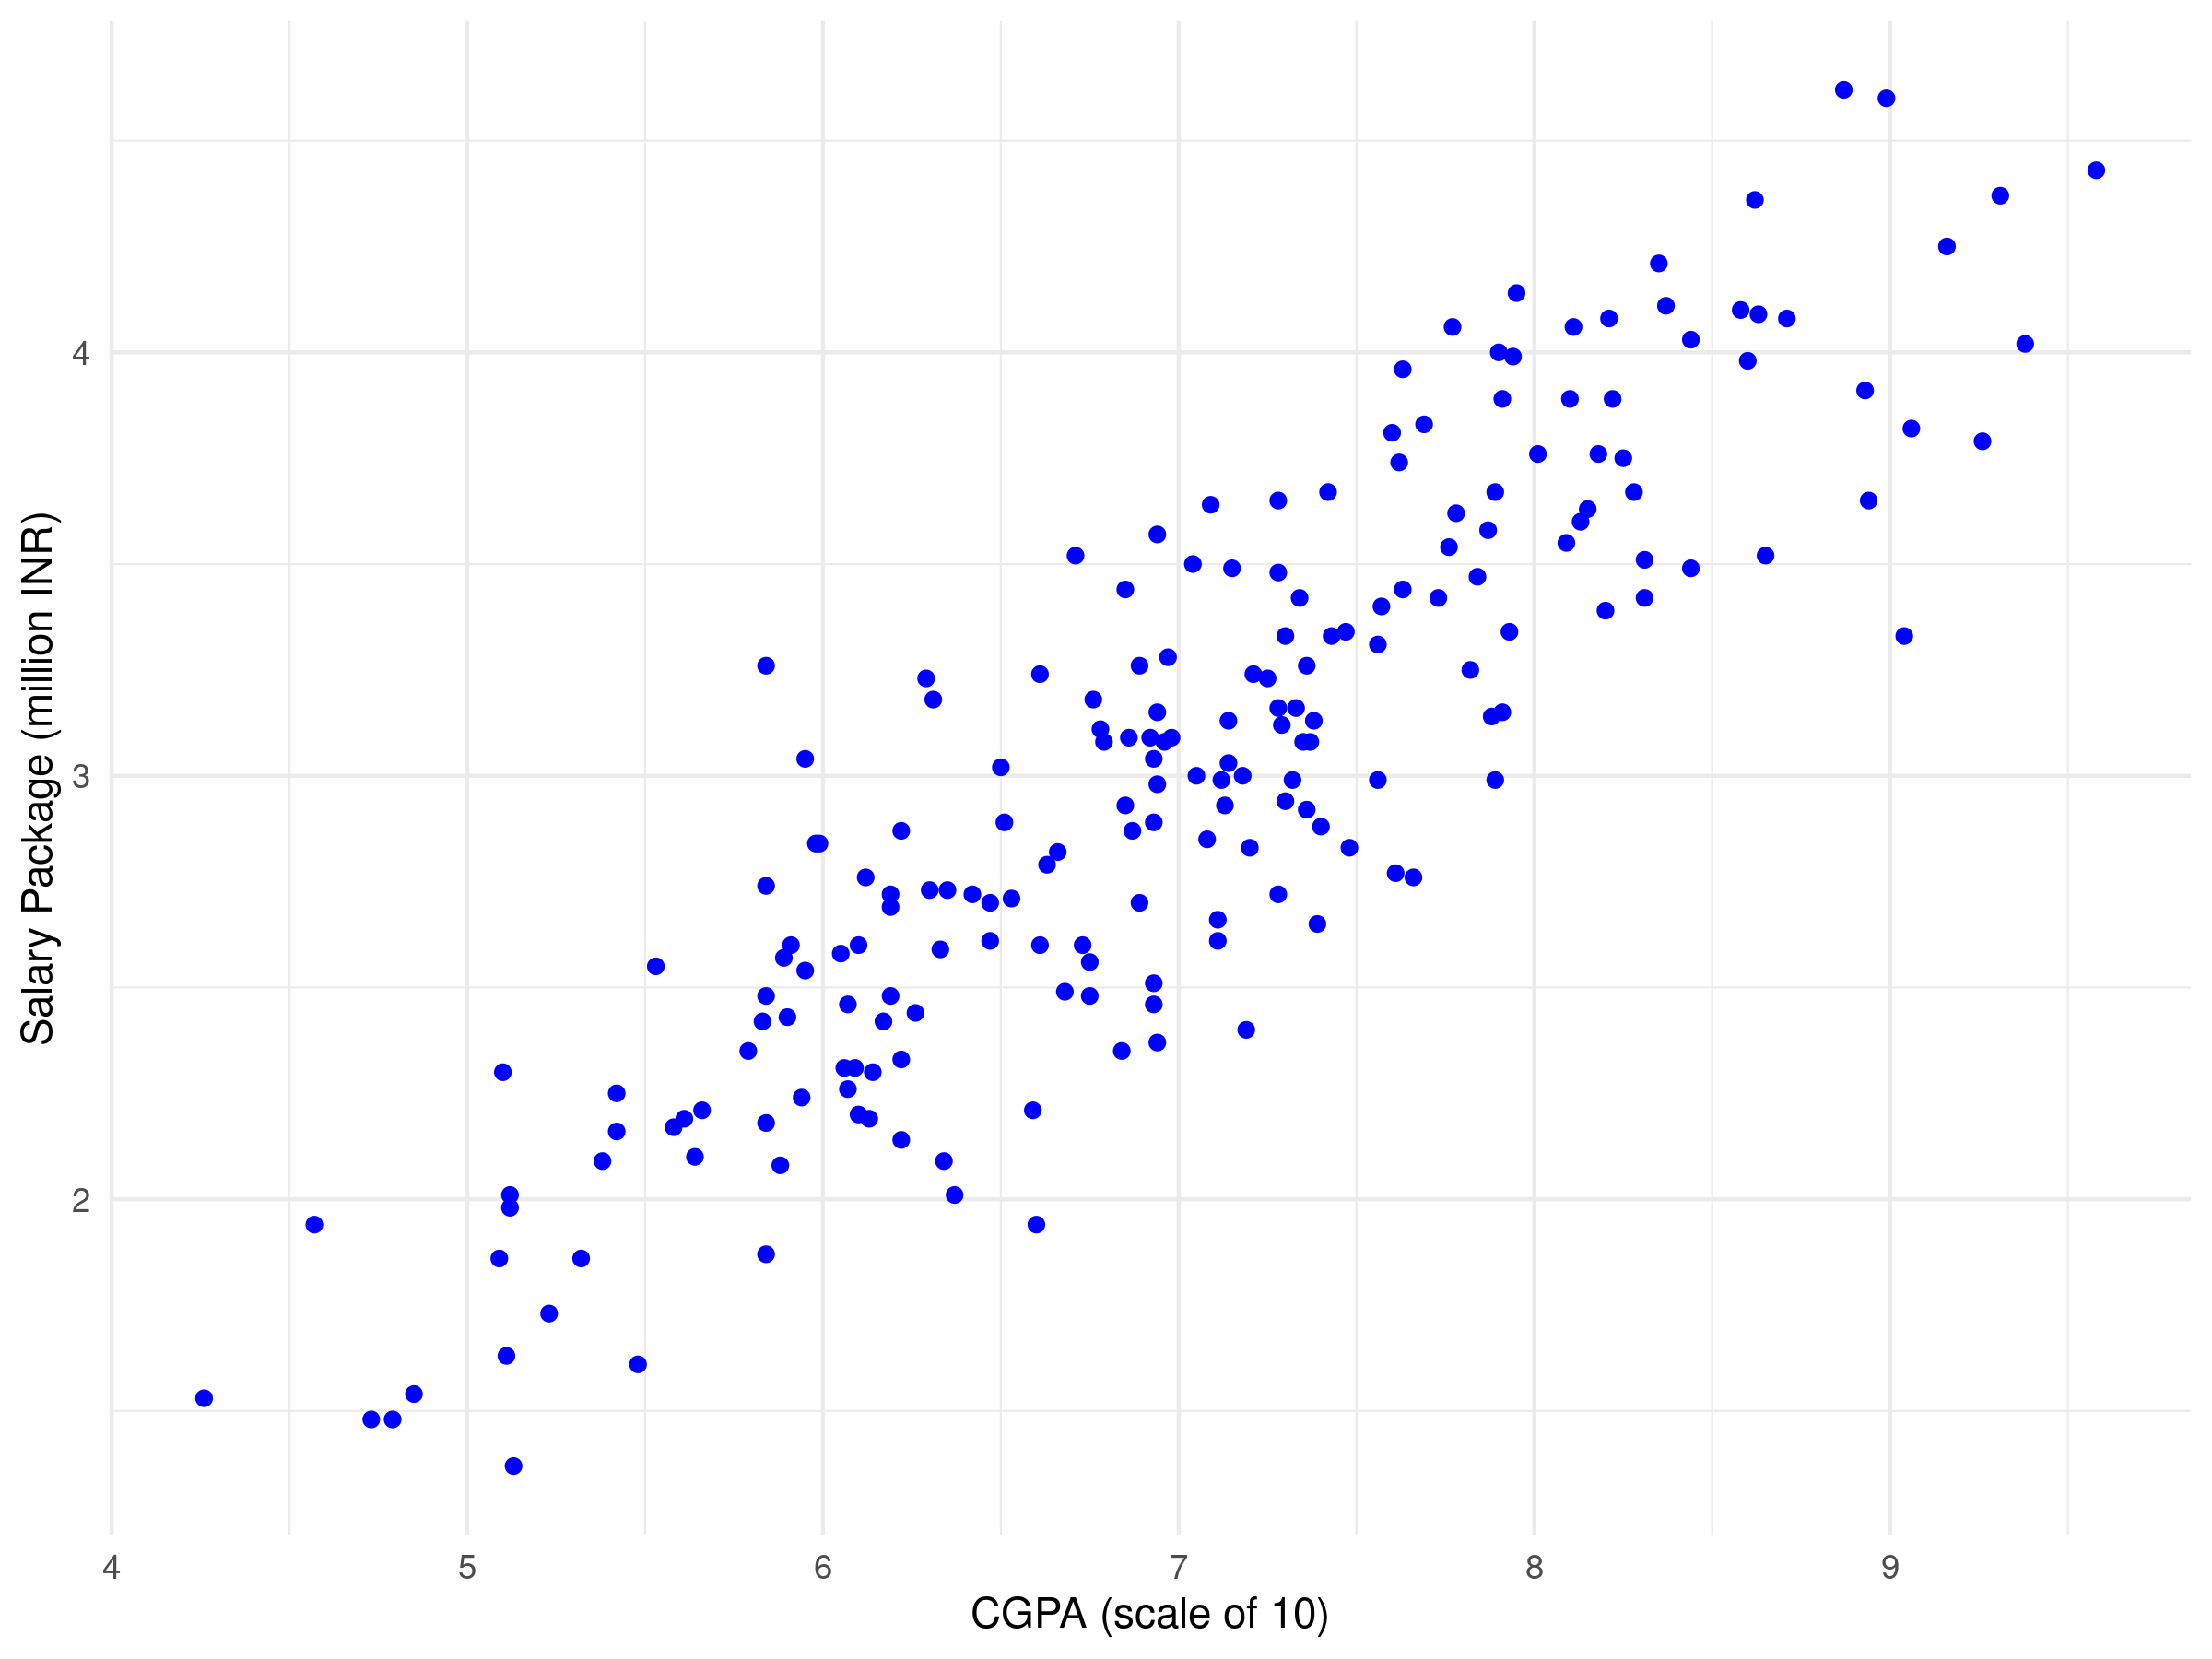
\includegraphics[width=0.9\textwidth]{chapters/chapter1/plots/scatter_plot.png}
    \caption{Scatter Plot of CGPA vs Salary Package}
    \label{fig:scatter_plot_cgpa_salary}
\end{figure}

\begin{definition}
    Regression is a statistical method used to establish the relationship between a dependent variable and one or more independent variables. It allows us to make predictions about the dependent variable based on the values of the independent variables. In our case, we are specifically focusing on simple linear regression, which involves one dependent variable and one independent variable.
\end{definition}

Once we have our training data, we can use it to estimate the coefficients \(\hat{\beta}_0\) and \(\hat{\beta}_1\) for our linear model. These estimated coefficients allow us to predict the average salary package for a given CGPA. The prediction can be expressed as:

\[
\hat{Y} = \hat{\beta}_0 + \hat{\beta}_1 X
\]

In this equation, \(\hat{Y}\) represents the predicted value of the salary package \(Y\) based on the given CGPA \(x\). The parameter \(\hat{\beta}_1\) indicates the expected increase in the salary package for each one-unit increase in CGPA.

\subsection{Estimating the Coefficients}

To evaluate the fit of our linear regression model, we define the \textbf{Sum of Squared Residuals (SSR)}. SSR quantifies the discrepancy between the observed values and the values predicted by our model. \\

Mathematically, it is expressed as:

\[
\text{SSR} = \sum_{i=1}^{n} (y_i - \hat{y}_i)^2
\]

where:\\
\(y_i\) is the observed value of the dependent variable (salary package),\\
\(\hat{y}_i\) is the predicted value of the dependent variable based on our regression model,\\
\(n\) is the number of observations.\\

The objective of linear regression is to minimize the SSR, leading us to the best-fitting line. To derive the estimates of the coefficients \(\hat{\beta}_0\) and \(\hat{\beta}_1\), we start with the linear model equation:

\[
Y = \beta_0 + \beta_1 X_1 + \epsilon
\]

The predicted values \(\hat{Y}\) can be written as:

\[
\hat{Y} = \hat{\beta}_0 + \hat{\beta}_1 X_1
\]

To estimate the coefficients, we need to minimize the SSR. We can substitute \(\hat{Y}\) into the SSR formula:

\[
\text{SSR} = \sum_{i=1}^{n} \left( y_i - \left( \hat{\beta}_0 + \hat{\beta}_1 x_{i} \right) \right)^2
\]

To find the values of \(\hat{\beta}_0\) and \(\hat{\beta}_1\) that minimize the SSR, we take the partial derivatives of SSR with respect to \(\hat{\beta}_0\) and \(\hat{\beta}_1\), set them to zero, and solve the resulting equations.\\

First, we calculate the derivative with respect to \(\hat{\beta}_1\):

\[
\frac{\partial \text{SSR}}{\partial \hat{\beta}_1} = -2 \sum_{i=1}^{n} (y_i - \hat{\beta}_0 - \hat{\beta}_1 x_i) x_i
\]

Setting this derivative to zero:

\[
-2 \sum_{i=1}^{n} (y_i - \hat{\beta}_0 - \hat{\beta}_1 x_i) x_i = 0
\]

This simplifies to:

\[
\sum_{i=1}^{n} (y_i - \hat{\beta}_0 - \hat{\beta}_1 x_i) x_i = 0
\]

\vspace{8pt}
Next, we calculate the derivative with respect to \(\hat{\beta}_0\):

\[
\frac{\partial \text{SSR}}{\partial \hat{\beta}_0} = -2 \sum_{i=1}^{n} (y_i - \hat{\beta}_0 - \hat{\beta}_1 x_i)
\]

Setting this derivative to zero gives us:

\[
-2 \sum_{i=1}^{n} (y_i - \hat{\beta}_0 - \hat{\beta}_1 x_i) = 0
\]

This simplifies to:

\[
\sum_{i=1}^{n} (y_i - \hat{\beta}_0 - \hat{\beta}_1 x_i) = 0
\]

From the above two equations, we have:\\

1. 
\[
\sum_{i=1}^{n} y_i = n\hat{\beta}_0 + \hat{\beta}_1 \sum_{i=1}^{n} x_i 
\]

2. 
\[
\sum_{i=1}^{n} y_i x_i = \hat{\beta}_0 \sum_{i=1}^{n} x_i + \hat{\beta}_1 \sum_{i=1}^{n} x_i^2
\]

Next, we express \(\hat{\beta}_0\) in terms of \(\hat{\beta}_1\) using the first equation:

\[
n\hat{\beta}_0 = \sum_{i=1}^{n} y_i - \hat{\beta}_1 \sum_{i=1}^{n} x_i
\]

Now we take the second normal equation:

\[
\sum_{i=1}^{n} y_i x_i = \hat{\beta}_0 \sum_{i=1}^{n} x_i + \hat{\beta}_1 \sum_{i=1}^{n} x_i^2
\]

Substituting the expression for \(\hat{\beta}_0\) we obtained:

\[
\sum_{i=1}^{n} y_i x_i = \left( \frac{\sum_{i=1}^{n} y_i - \hat{\beta}_1 \sum_{i=1}^{n} x_i}{n} \right) \sum_{i=1}^{n} x_i + \hat{\beta}_1 \sum_{i=1}^{n} x_i^2
\]

To solve for \(\hat{\beta}_1\), we can express it as:

\[
\hat{\beta}_1 = \frac{n\sum_{i=1}^{n} y_i x_i - \sum_{i=1}^{n} y_i \sum_{i=1}^{n} x_i}{n\sum_{i=1}^{n} x_i^2 - \left( \sum_{i=1}^{n} x_i \right)^2} \tag{1.2}
\]

Finally, substituting \(\hat{\beta}_1\) back into the equation for \(\hat{\beta}_0\), we can obtain:

\[
\hat{\beta}_0 = \frac{1}{n}\sum_{i=1}^{n} y_i - \hat{\beta}_1 \cdot \frac{1}{n}\sum_{i=1}^{n} x_i \tag{1.3}
\]

\subsubsection{Simplication of above formulas}

To simplify the formulas for \(\hat{\beta}_1\) and \(\hat{\beta}_0\) around the mean of \(X\) and \(Y\), we define the means as follows:

\[
\bar{x} = \frac{1}{n}\sum_{i=1}^{n} x_i \quad \text{and} \quad \bar{y} = \frac{1}{n}\sum_{i=1}^{n} y_i.
\]

Starting with the formula for \(\hat{\beta}_1\):

\[
\hat{\beta}_1 = \frac{n\sum_{i=1}^{n} y_i x_i - \sum_{i=1}^{n} y_i \sum_{i=1}^{n} x_i}{n\sum_{i=1}^{n} x_i^2 - \left( \sum_{i=1}^{n} x_i \right)^2},
\]

we denote:

\[
S_{xy} = \sum_{i=1}^{n} (y_i - \bar{y})(x_i - \bar{x}) \quad \text{and} \quad S_{xx} = \sum_{i=1}^{n} (x_i - \bar{x})^2.
\]

Thus, we can express \(\hat{\beta}_1\) as:

\[
\hat{\beta}_1 = \frac{S_{xy}}{S_{xx}}.
\]

Expanding \(S_{xy}\):

\[
S_{xy} = \sum_{i=1}^{n} y_i x_i - n\bar{y}\bar{x}.
\]

Expanding \(S_{xx}\):

\[
S_{xx} = \sum_{i=1}^{n} x_i^2 - n\bar{x}^2.
\]

Substituting \(S_{xy}\) and \(S_{xx}\) into \(\hat{\beta}_1\):

\[
\hat{\beta}_1 = \frac{\sum_{i=1}^{n} y_i x_i - n\bar{y}\bar{x}}{\sum_{i=1}^{n} x_i^2 - n\bar{x}^2}.
\]

Now, for \(\hat{\beta}_0\):

\[
\hat{\beta}_0 = \bar{y} - \hat{\beta}_1 \bar{x}.
\]

Substituting \(\hat{\beta}_1\) into the formula gives:

\[
\hat{\beta}_0 = \bar{y} - \frac{S_{xy}}{S_{xx}} \bar{x}.
\]

Thus, the simplified forms for the regression coefficients are:

\[
\hat{\beta}_1 = \frac{S_{xy}}{S_{xx}} \quad \text{and} \quad \hat{\beta}_0 = \bar{y} - \hat{\beta}_1 \bar{x}.
\]

\vspace{12pt}
By applying the derived formulas for the coefficients on the dataset shared, we obtain the estimates:

\[
\hat{\beta}_0 = -0.98568 \quad \text{and} \quad \hat{\beta}_1 = 0.56959
\]

With these estimates, we can represent the linear regression model as:

\[
\hat{Y} = -0.98568 + 0.56959 X
\]

This equation indicates that for each unit increase in the single observation of CGPA (\(x\)), the salary package (\(y\)) is expected to increase by approximately 0.56959 million INR per annum, while the intercept suggests that the predicted salary package approaches -0.98568 million INR when the CGPA is zero. This simply implies CGPA should be at a certain threshold to start earning (which affirms you only get a job if you pass!) \\

To visualize how well this linear model fits our data, we can plot the regression line on the scatter plot created earlier, which shows the relationship between CGPA and salary package [\ref{fig:scatter_plot_cgpa_salary_with_lm}]. The scatter plot effectively demonstrates the positive correlation, and overlaying the regression line illustrates the predicted values based on our model coefficients. 

\begin{figure}[h!]
    \centering
    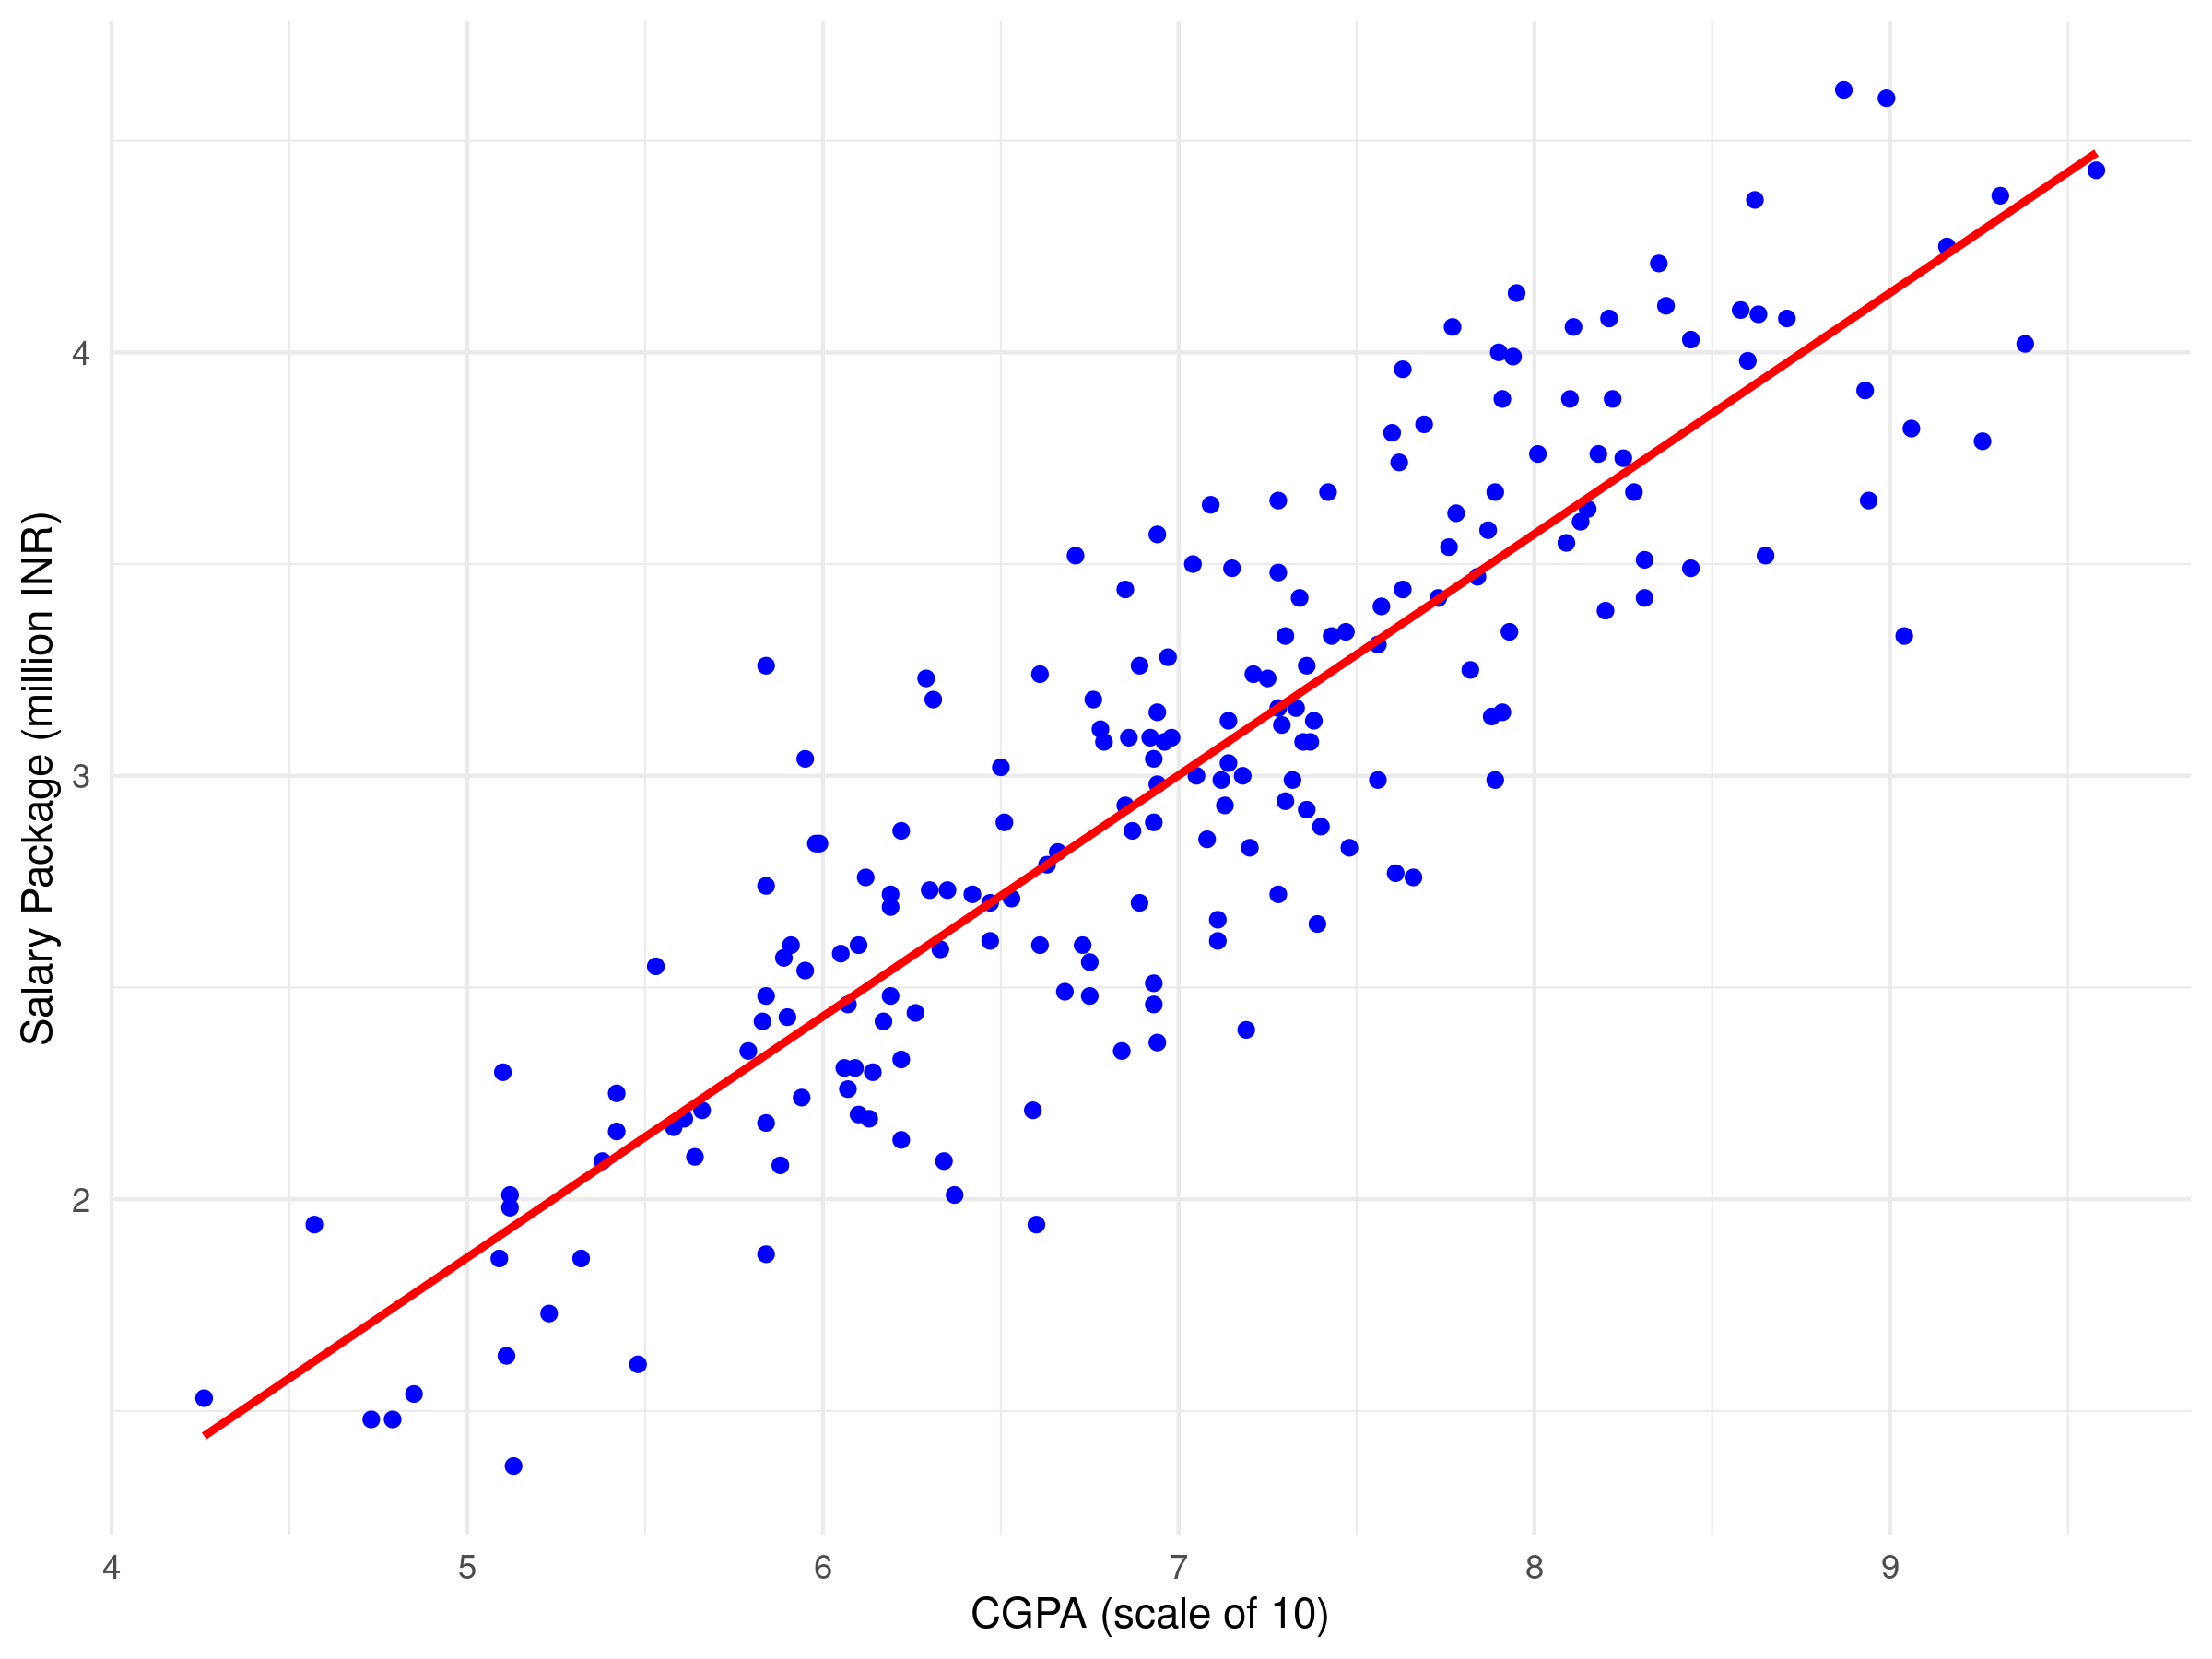
\includegraphics[width=0.9\textwidth]{chapters/chapter1/plots/scatter_plot_with_lm.png}
    \caption{Scatter Plot of CGPA vs Salary Package with Simple Linear Regression Line}
    \label{fig:scatter_plot_cgpa_salary_with_lm}
\end{figure}

\subsection{Assessing the Accuracy of the Coefficients Estimates}

Recall that we assume the true relationship between the independent variable \(X\) and the dependent variable \(Y\) can be expressed in the form 

\[
Y = f(X) + \epsilon
\]

where \(f\) is an unknown function and \(\epsilon\) represents a mean-zero random error term that follows a normal distribution. The error term \(\epsilon\) acts as a catch-all for various factors that are not captured by this simplified model. In reality, the true relationship between \(X\) and \(Y\) is likely to be nonlinear, and there may be additional variables influencing \(Y\) that we have not considered. Furthermore, measurement error may also contribute to the discrepancies observed in our model predictions.\\

A crucial assumption in linear regression is that the error term \(\epsilon\) is independent of the independent variable \(X\). This independence allows us to make valid inferences about the parameters of our model.\\

In the context of regression analysis, it is essential to differentiate between population coefficients and sample coefficients. The population coefficients, often denoted as \(\beta_0\) and \(\beta_1\), represent the true parameters in the population we wish to estimate. In contrast, sample coefficients, represented as \(\hat{\beta}_0\) and \(\hat{\beta}_1\), are computed from the sample data and serve as estimates of the population coefficients.\\

An estimator is said to be unbiased if its expected value equals the true parameter value. In other words, an estimator \(\hat{\beta}\) is unbiased if 

\[
E[\hat{\beta}] = \beta.
\]

This implies that, on average, the estimator will yield the correct value for the parameter over numerous samples. \\

\begin{theorem}
    $\hat{\beta}_1$ and $\hat{\beta}_0$ are unbiased estimators of $\beta_1$ and $\beta_0$.
\end{theorem}

\begin{proof}
    We start with 
    \[
y_i = \beta_0 + \beta_1 x_i + \epsilon_i,
\]

The OLS estimate for the slope \(\hat{\beta}_1\) is given by:

\[
\hat{\beta}_1 = \frac{\sum_{i=1}^n (x_i - \bar{x})(y_i - \bar{y})}{\sum_{i=1}^n (x_i - \bar{x})^2}.
\]

Substituting \(y_i\):

\[
\hat{\beta}_1 = \frac{\sum_{i=1}^n (x_i - \bar{x})\left(\beta_0 + \beta_1 x_i + \epsilon_i - \bar{y}\right)}{\sum_{i=1}^n (x_i - \bar{x})^2}.
\]

Noting that \(\bar{y} = \beta_0 + \beta_1 \bar{x}\), we have:

\[
\hat{\beta}_1 = \beta_1 + \frac{\sum_{i=1}^n (x_i - \bar{x}) \epsilon_i}{\sum_{i=1}^n (x_i - \bar{x})^2}.
\]

Taking expectations gives:

\[
E[\hat{\beta}_1] = \beta_1 + E\left[\frac{\sum_{i=1}^n (x_i - \bar{x}) \epsilon_i}{\sum_{i=1}^n (x_i - \bar{x})^2}\right].
\]

Since \(E[\epsilon_i] = 0\), it follows that:

\[
E[\hat{\beta}_1] = \beta_1 + 0 = \beta_1.
\]

Using:

\[
\hat{\beta}_0 = \bar{y} - \hat{\beta}_1 \bar{x},
\]

and taking expectations:

\[
E[\hat{\beta}_0] = E[\bar{y}] - E[\hat{\beta}_1] \bar{x}.
\]

Thus:

\[
E[\hat{\beta}_0] = \beta_0 + \beta_1 \bar{x} - \beta_1 \bar{x} = \beta_0.
\]
\end{proof}


This means that both sample coefficients are unbiased estimators of their respective population coefficients. \\

The variances of the estimators \(\hat{\beta}_0\) and \(\hat{\beta}_1\) provide insight into the variability of these estimates across different samples. 

\begin{theorem}
    The variance of the estimator \(\hat{\beta}_0\) in a simple linear regression model is given by:

\[
Var(\hat{\beta}_0) = \sigma^2 \left( \frac{1}{n} + \frac{\bar{x}^2}{\sum (x_i - \bar{x})^2} \right),
\]

where \(\sigma^2\) is the variance of the error term, \(n\) is the sample size, \(\bar{x}\) is the mean of the independent variable \(x\), and \(x_i\) represents individual observations of \(x\).
\end{theorem}

\begin{proof}
    Consider the simple linear regression model given by:

\[
y_i = \beta_0 + \beta_1 x_i + \epsilon_i,
\]

where \(\epsilon_i\) are independent and identically distributed (i.i.d.) error terms with mean zero and variance \(\sigma^2\). \\

The ordinary least squares (OLS) estimates of the coefficients \(\hat{\beta}_0\) and \(\hat{\beta}_1\) are given by:

\[
\hat{\beta}_1 = \frac{\sum (x_i - \bar{x})(y_i - \bar{y})}{\sum (x_i - \bar{x})^2},
\]

and

\[
\hat{\beta}_0 = \bar{y} - \hat{\beta}_1 \bar{x}.
\]

To derive \(Var(\hat{\beta}_0)\), we first express \(\hat{\beta}_0\) in terms of \(y_i\):

\[
\hat{\beta}_0 = \bar{y} - \hat{\beta}_1 \bar{x}.
\]

Next, we need the variance of \(\hat{\beta}_0\):

\[
Var(\hat{\beta}_0) = Var(\bar{y} - \hat{\beta}_1 \bar{x}).
\]

Since \(\bar{x}\) is a constant, we have:

\[
Var(\hat{\beta}_0) = Var(\bar{y}) + \bar{x}^2 Var(\hat{\beta}_1).
\]

The variance of the sample mean \(\bar{y}\) is given by:

\[
Var(\bar{y}) = \frac{\sigma^2}{n}.
\]

Now, we need to calculate \(Var(\hat{\beta}_1)\):

\[
Var(\hat{\beta}_1) = \frac{\sigma^2}{\sum (x_i - \bar{x})^2}.
\]

Substituting this into our equation for \(Var(\hat{\beta}_0)\):

\[
Var(\hat{\beta}_0) = \frac{\sigma^2}{n} + \bar{x}^2 \left( \frac{\sigma^2}{\sum (x_i - \bar{x})^2} \right).
\]

Factoring out \(\sigma^2\):

\[
Var(\hat{\beta}_0) = \sigma^2 \left( \frac{1}{n} + \frac{\bar{x}^2}{\sum (x_i - \bar{x})^2} \right).
\]
\end{proof}

The variance formula for the estimator \(\hat{\beta}_0\) indicates how much uncertainty exists in the intercept estimate of a linear regression model. A lower variance suggests more reliable estimates, emphasizing the importance of larger sample sizes and diverse data points to enhance prediction accuracy. It helps practitioners understand the trade-offs between error variability and data characteristics, guiding better decision-making in model development and interpretation.

\begin{theorem}
    The variance of the estimator \(\hat{\beta}_1\) in a simple linear regression model can be expressed as:

\[
Var(\hat{\beta}_1) = \frac{\sigma^2}{\sum (x_i - \bar{x})^2}
\]
\end{theorem}

\begin{proof}
    We start with the linear regression model:

   \[
   y_i = \beta_0 + \beta_1 x_i + \epsilon_i
   \]

   where \(\epsilon_i\) are independent and identically distributed (i.i.d.) error terms with mean zero and variance \(\sigma^2\). \\

   The estimator for \(\beta_1\) is given by:

   \[
   \hat{\beta}_1 = \frac{\sum (x_i - \bar{x})(y_i - \bar{y})}{\sum (x_i - \bar{x})^2}
   \]

   Substitute \(y_i\) from the model into the estimator:

   \[
   \hat{\beta}_1 = \frac{\sum (x_i - \bar{x})(\beta_0 + \beta_1 x_i + \epsilon_i - \bar{y})}{\sum (x_i - \bar{x})^2}
   \]

   Simplifying, we focus on the terms involving \(\epsilon_i\):

   \[
   \hat{\beta}_1 = \beta_1 + \frac{\sum (x_i - \bar{x}) \epsilon_i}{\sum (x_i - \bar{x})^2}
   \]

   To find \(Var(\hat{\beta}_1)\), we use the properties of variance. Since the \(x_i\) values are fixed, we focus on the variability introduced by \(\epsilon_i\):

   \[
   Var(\hat{\beta}_1) = Var\left(\frac{\sum (x_i - \bar{x}) \epsilon_i}{\sum (x_i - \bar{x})^2}\right)
   \]

   Given that the \(\epsilon_i\) are independent and have variance \(\sigma^2\), we have:

   \[
   Var(\hat{\beta}_1) = \frac{\sum (x_i - \bar{x})^2 Var(\epsilon_i)}{(\sum (x_i - \bar{x})^2)^2} = \frac{\sigma^2}{\sum (x_i - \bar{x})^2}
   \]

\end{proof}

This formula indicates that the precision of the slope estimate \(\hat{\beta}_1\) improves with greater variability in the predictor \(x\) and larger sample sizes. For these formulas to be strictly valid, we assume that the errors \(\epsilon_i\) are uncorrelated with a common variance \(\sigma^2\); while this assumption may not always hold, the formulas still provide a good approximation.

\subsection{Reliability of the Estimators}

Reliability refers to how accurately an estimator can approximate the true parameter values. Key aspects of estimator reliability include confidence intervals, hypothesis testing, and the calculation of the t-statistic.\\

We start it by defining the standard error (SE).

\begin{definition}
    The standard error (SE) indicates the variability of the estimator from sample to sample. The standard error is calculated as the square root of the estimated variance of the estimator:

\[
SE(\hat{\beta}) = \sqrt{Var(\hat{\beta})}
\]

where \(Var(\hat{\beta})\) is the variance of the estimator \(\hat{\beta}\). The standard error plays a critical role in determining how far the sample estimates are likely to be from the true population parameters. A smaller standard error indicates that the estimate is more reliable and that it is likely to be closer to the true parameter value.
\end{definition}

For instance, if the variance of an estimator \(\hat{\beta}\) is calculated to be \(0.04\), the standard error is:

\[
SE(\hat{\beta}) = \sqrt{0.04} = 0.2
\]

This indicates that the estimator \(\hat{\beta}\) is expected to vary by \(0.2\) units around the true parameter value across different samples.

\begin{example}
    For our CGPA vs Salary Package dataset, the results look like this: \\

    \textbf{Standard Error of Intercept (\(SE(\hat{\beta}_0)\))}: 0.15396\\
    \textbf{Standard Error of CGPA (\(SE(\hat{\beta}_1)\))}: 0.02177\\

    These values indicates the average distance that the estimated parameters are expected to be from the true population parameters. A smaller standard error suggests that the estimate is more precise.
\end{example}

\begin{definition}
    A confidence interval provides a range of values within which we can expect the true parameter to lie, with a certain level of confidence. For instance, a 95\% confidence interval for the parameter \(\beta\) in a regression model is calculated as:

\[
\hat{\beta} \pm t_{\alpha/2, n-2} \cdot SE(\hat{\beta})
\]

where:
\begin{itemize}
    \item \(\hat{\beta}\) is the estimated parameter,
    \item \(t_{\alpha/2, n-2}\) is the critical value from the t-distribution for a given significance level \(\alpha\) and \(n-2\) degrees of freedom,
    \item \(SE(\hat{\beta})\) is the standard error of the estimator.
\end{itemize}
\end{definition}

For example, if \(\hat{\beta}_1 = 1.5\) and \(SE(\hat{\beta}_1) = 0.3\) with \(n = 30\), the critical value for a 95\% confidence interval (approximately \(t_{0.025, 28} \approx 2.048\)) leads to:

\[
1.5 \pm 2.048 \cdot 0.3 \implies [0.608, 2.392]
\]

This interval suggests that we can be 95\% confident that the true value of \(\beta_1\) lies between 0.608 and 2.392. The smaller this interval, the better. 

\begin{example}
    For our CGPA vs Salary Package dataset, we use the formula:

    \[
    \text{Confidence Interval} = \hat{\beta} \pm t_{\alpha/2, n-2} \times SE(\hat{\beta})
    \]
    
    Assuming a typical critical t-value for 95\% confidence and 98 degrees of freedom (approximately \(1.984\)), we calculate:\\

    \textbf{For \(\hat{\beta}_0\)}:
\[
\text{CI for } \hat{\beta}_0 = -0.98568 \pm 1.984 \times 0.15396
\]
\[
\text{CI} = [-1.29113664, -0.68022336]
\]

\textbf{For \(\hat{\beta}_1\)}:
\[
\text{CI for } \hat{\beta}_1 = 0.56959 \pm 1.984 \times 0.02177
\]
\[
\text{CI} = [0.52639832, 0.61278168]
\]
\end{example}

\subsubsection{Hypothesis Testing of Parameters}

Hypothesis testing allows us to assess whether the evidence in our data is strong enough to reject a null hypothesis \(H_0\) in favor of an alternative hypothesis \(H_1\). For linear regression, the null hypothesis typically states that the parameter equals zero (no effect).\\

The test statistic is calculated as:

\[
t = \frac{\hat{\beta} - \beta_0}{SE(\hat{\beta})}
\]

where \(\beta_0\) is the value under the null hypothesis (usually 0). It quantifies the distance between the estimated parameter and the hypothesized value, scaled by the standard error, providing reliable conclusions from empirical data. The calculated \(t\) statistic is then compared against the critical values from the t-distribution to determine whether to reject \(H_0\).\\

For example, if \(\hat{\beta}_1 = 1.5\) and \(SE(\hat{\beta}_1) = 0.3\), the t-statistic is:

\[
t = \frac{1.5 - 0}{0.3} = 5
\]

If our critical value for \(t_{0.025, n-2}\) is 2.048, we can reject the null hypothesis since \(5 > 2.048\), indicating that the predictor significantly affects the response variable.\\

\textit{Why t-statistic?}\\

The t-statistic is used in statistical inference, particularly for small sample sizes (typically \(n < 30\)), where the population standard deviation is unknown. It adjusts for the extra uncertainty from estimating the sample standard deviation, making it more conservative than the z-statistic. As the sample size increases, the t-distribution approaches the standard normal distribution. The t-statistic assumes normally distributed errors in the model, allowing for valid hypothesis testing and the construction of confidence intervals.

\begin{example}
    \textbf{Null and Alternative Hypotheses:}
\begin{itemize}
    \item \textbf{Null Hypothesis (\(H_0\))}: The coefficient is equal to zero (no effect).
    \begin{itemize}
        \item \(H_0: \hat{\beta}_1 = 0\) (CGPA has no effect on salary package)
    \end{itemize}
    \item \textbf{Alternative Hypothesis (\(H_a\))}: The coefficient is not equal to zero (there is an effect).
    \begin{itemize}
        \item \(H_a: \hat{\beta}_1 \neq 0\)
    \end{itemize}
\end{itemize}

The t-value for CGPA is 26.162, and the p-value is $< 2^{-16}$.\\

Since the p-value is far less than the common significance level of 0.05 and t-value is far above 2.048, we reject the null hypothesis.
\end{example}

\subsection{How good is the model?}

When assessing how well a regression model fits the data, three crucial metrics often used are the Residual Standard Error (RSE), the \(R^2\) value and the F-statistic. These metrics help quantify the model's accuracy and the amount of variability explained by the predictors.

\begin{definition}
    The Residual Standard Error (RSE) provides an estimate of the standard deviation of the residuals, which are the differences between observed values and the values predicted by the model. It is calculated using the formula:

\[
\text{RSE} = \sqrt{\frac{1}{n-2} \sum_{i=1}^{n} (y_i - \hat{y}_i)^2}
\]

where:\\
\(y_i\) is the observed value,\\
\(\hat{y}_i\) is the predicted value,\\
\(n\) is the number of observations.
\end{definition}

The RSE serves as a measure of how well the model predictions match the actual data. A smaller RSE indicates a better fit, as it suggests that the residuals (errors) are small and the predictions are close to the actual values. It provides an intuitive understanding of the average prediction error in the units of the response variable.

\begin{definition}
    The \(R^2\) value, also known as the coefficient of determination, quantifies the proportion of the variance in the dependent variable that can be explained by the independent variable(s) in the model. The \(R^2\) value is calculated using the formula:
    
    \[
    R^2 = 1 - \frac{\text{SS}_{\text{res}}}{\text{SS}_{\text{tot}}}
    \]

    where:
    \begin{description}
        \item[\(\text{SS}_{\text{res}}\)] is the residual sum of squares:
        \[
        \text{SS}_{\text{res}} = \sum_{i=1}^{n} (y_i - \hat{y}_i)^2
        \]
        
        \item[\(\text{SS}_{\text{tot}}\)] is the total sum of squares:
        \[
        \text{SS}_{\text{tot}} = \sum_{i=1}^{n} (y_i - \bar{y})^2
        \]
        
        \item[\(\bar{y}\)] is the mean of the observed values.
    \end{description}
\end{definition}

An \(R^2\) value of 1 indicates that the model explains all the variability of the response data around its mean, whereas an \(R^2\) value of 0 indicates that the model explains none of the variability. \\

While \(R^2\) is a useful measure, it has its limitations. One significant issue is that \(R^2\) always increases when additional predictors are added to the model, regardless of whether those predictors are truly relevant. This can lead to overfitting, where the model becomes too complex and captures noise rather than the underlying relationship.\\

To address this limitation, we often turn to the Adjusted \(R^2\), which adjusts the \(R^2\) value based on the number of predictors in the model. 

\begin{definition} The Adjusted \( R^2 \) is defined mathematically as:
    \[
\text{Adjusted } R^2 = 1 - \left( \frac{(1 - R^2)(n - 1)}{n - p - 1} \right)
\]

where \(p\) is the number of predictors in the model.
\end{definition}

The Adjusted \(R^2\) provides a more accurate measure of goodness-of-fit by penalizing the addition of unnecessary predictors. A higher Adjusted \(R^2\) indicates a better fit, while accounting for the complexity of the model.\\

The F-statistic is a crucial metric in regression analysis, particularly when evaluating the overall significance of a linear regression model. It helps to determine whether the independent variable(s) in the model explain a significant portion of the variance in the dependent variable. \\

\begin{definition}
    The F-statistic is calculated as follows:

    \[
    F = \frac{\text{MS}_{\text{regression}}}{\text{MS}_{\text{residual}}}
    \]

    where:
    \begin{align*}
    \text{MS}_{\text{regression}} & = \frac{\text{SS}_{\text{regression}}}{p - 1}, \\
    \text{MS}_{\text{residual}} & = \frac{\text{SS}_{\text{residual}}}{n - p}.
    \end{align*}

    In these formulas:
    \begin{itemize}
        \item \(\text{SS}_{\text{regression}}\) is the sum of squares due to regression, which measures the variation explained by the regression model.
        \item \(\text{SS}_{\text{residual}}\) is the sum of squares of the residuals, which measures the variation not explained by the model.
        \item \(p\) is the number of predictors (including the intercept).
        \item \(n\) is the number of observations.
    \end{itemize}
\end{definition}

\textbf{Calculation Steps:}

\begin{enumerate}
    \item \textit{Calculate Total Sum of Squares (\(SS_{\text{total}}\))}:
    \[
    SS_{\text{total}} = \sum_{i=1}^{n}(y_i - \bar{y})^2
    \]
    where \(\bar{y}\) is the mean of the dependent variable.

    \item \textit{Calculate Regression Sum of Squares (\(SS_{\text{regression}}\))}:
    \[
    SS_{\text{regression}} = \sum_{i=1}^{n}(\hat{y}_i - \bar{y})^2
    \]
    where \(\hat{y}_i\) is the predicted value from the regression model.

    \item \textit{Calculate Residual Sum of Squares (\(SS_{\text{residual}}\))}:
    \[
    SS_{\text{residual}} = \sum_{i=1}^{n}(y_i - \hat{y}_i)^2
    \]

    \item \textit{Compute Mean Squares}:
    \[
    \text{MS}_{\text{regression}} = \frac{SS_{\text{regression}}}{p - 1}, \quad \text{MS}_{\text{residual}} = \frac{SS_{\text{residual}}}{n - p}
    \]

    \item \textit{Compute the F-Statistic}:
    \[
    F = \frac{\text{MS}_{\text{regression}}}{\text{MS}_{\text{residual}}}
    \]
\end{enumerate}

\textbf{Interpretation}:

\begin{itemize}
    \item The F-statistic tests the null hypothesis \(H_0: \beta_1 = 0\) (i.e., the independent variable does not explain any variance in the dependent variable) against the alternative hypothesis \(H_a: \beta_1 \neq 0\) (i.e., the independent variable explains some variance).
    \item A higher F-statistic value indicates that the model provides a better fit to the data than a model with no independent variables.
\end{itemize}

\begin{example}
    For our CGPA vs Salary Package dataset, the evaluation metrics are: 
    
    \begin{enumerate}
        \item \textbf{Residual Standard Error:} 0.3285 \\
        The residual standard error (RSE) indicates that, on average, the predicted salary packages deviate from the actual values by approximately 0.33 units. A smaller RSE suggests a good fit of the model.
        
        \item \textbf{Multiple R-squared:} 0.7756 \\
        This value implies that about 77.56\% of the variability in salary packages can be explained by CGPA, indicating a strong relationship between CGPA and salary.
        
        \item \textbf{Adjusted R-squared:} 0.7745 \\
        The adjusted R-squared is close to the multiple R-squared value, confirming that the model remains robust after accounting for the number of predictors.
        
        \item \textbf{F-statistic:} 684.4 on 1 and 198 DF \\
        The associated p-value is $< 2.2^{-16}$, indicating high statistical significance. This leads us to reject the null hypothesis, affirming that CGPA is a significant predictor of salary packages.
    \end{enumerate}
\end{example}
\section{Multiple Linear Regression}